\begin{frame}{Surface hexagonal structure appearance}
    \begin{columns}
    
    \column[T]{0.38\textwidth}

    \begin{overprint}
        \onslide<1>\begin{table}
            \centering
            \begin{tabular}{ |l|l|l|l| }
                \hline
                Argon & \ammonia & \dioxygen & Duration \\
                 & & & (hours) \\ 
                \hline
                50 & 0 & 0 & 24 \\
                42 & 0 & 8 & 12 \\
                41 & 1 & 8 & 5 \\
                \hline
                50 & 0 & 0 & 7 \\
                42 & 0 & 8 & 1 \\
                41 & 1 & 8 & 10 \\
                \rowcolor{shadecolor}
                48.5 & 1 & 0.5 & 13 \\
                49 & 1 & 0 & 11 \\
                50 & 0 & 0 & 8 \\
                \hline
            \end{tabular}
            \caption{Gas flow in reactor ($50$ mL/min, $0.3$ bar). In experimental order.}
        \end{table}
        \onslide<2>\begin{figure}
            \centering
            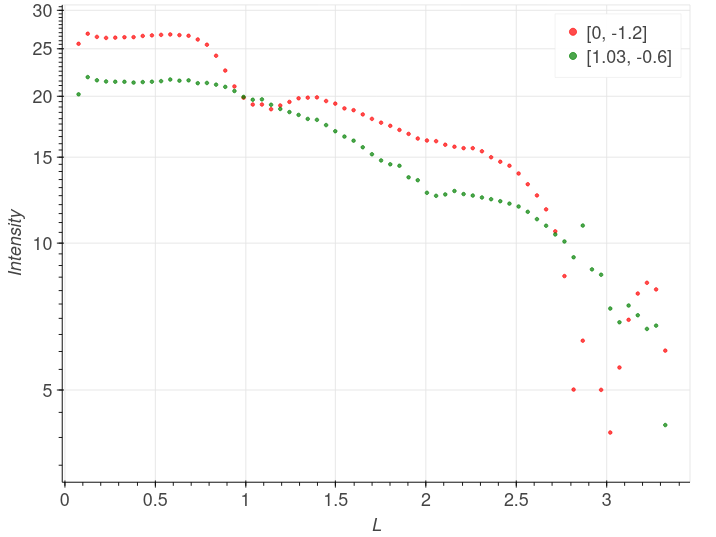
\includegraphics[width=\textwidth]{Figures/sxrd_data/ctr/reconstruction_ctr_condB.png}
            \caption{CTR on white diamond primary reflections. No structure in L can be easily identified, but rather a continuous decrease of the signal,  characteristic of an unordered structure in $\Vec{c}$.}
            \label{fig:ctr_conde}
        \end{figure}
    \end{overprint}

    Not hexagonal $\alpha-$Pt$O_2$ ($|\Vec{a}| \approx \SI{3.10}{\angstrom}$). Matches with (111) of \ptthreeofour. Primitive cell (red or white diamond) $a=4.624$.
    
    \column[T]{0.6\textwidth}
    
    \begin{figure}
        \centering
        % 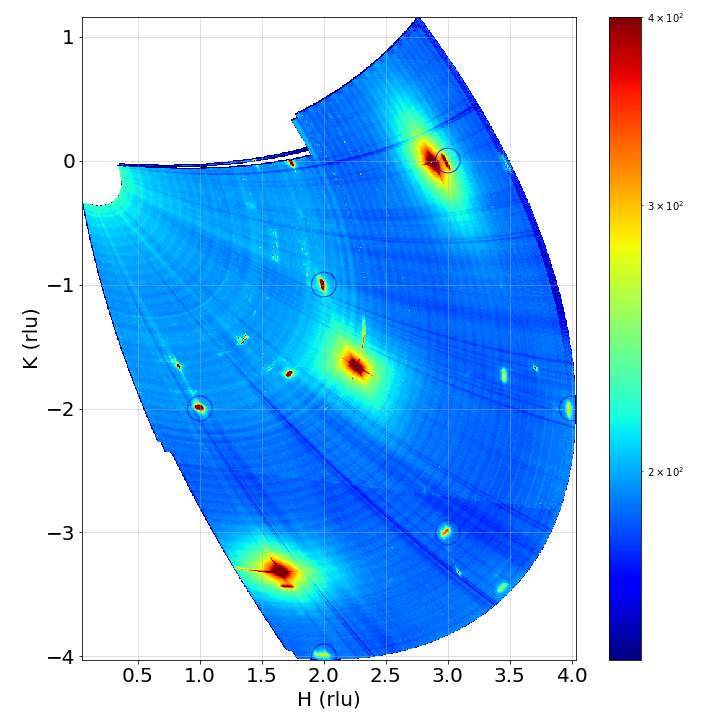
\includegraphics[width=0.85\textwidth, trim={14cm 0 3.5cm 0}, clip]{Figures/sxrd_data/maps/Map_hkl_surf_or_hex_2227-2283.png}

        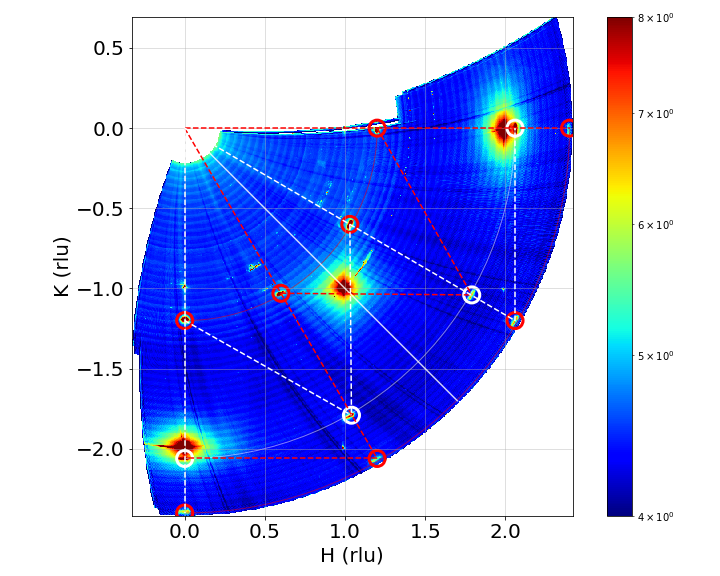
\includegraphics[trim=40 0 40 0, clip, width=0.95\textwidth]{Figures/sxrd_data/maps/Map_hkl_surf_or_2227-2283.png}
        \caption{Reciprocal space map. Atmospheres with low oxygen to ammonia ratio favour a hexagonal surface structure on Pt (100).}
        \label{fig:CondB}
    \end{figure}
    
    \end{columns}

\end{frame}